\documentclass{letter}

\usepackage[key]{fbtest}
\usepackage{fbpicture}
\usepackage{standalone}
\usepackage{amsmath}
\usepackage{graphicx}

\begin{document}

  \begin{problem}{}
    Our webapp uses the loading function $L(t) = \frac{1}{2}\sqrt{t}$.

    \subproblem{}{
      Find the loading time $l$ of our webapp.

      \solution{
        The loading speed $l$ is the at which the webapp is fully loaded.
        In other words, $l$ is the solution to $L(l) = 1$.

        \begin{align*}
          L(l) = 1 \\
          \frac{1}{2}\sqrt{l} = 1 \\
          l = 4
        \end{align*}
      }
    }

    \subproblem{}{
      Graph $L(t)$ on the domain $[0, l]$, and shade on the graph the
      region corresponding to the Google Speed Index of our webapp.

      \solution{
        \begin{center}
          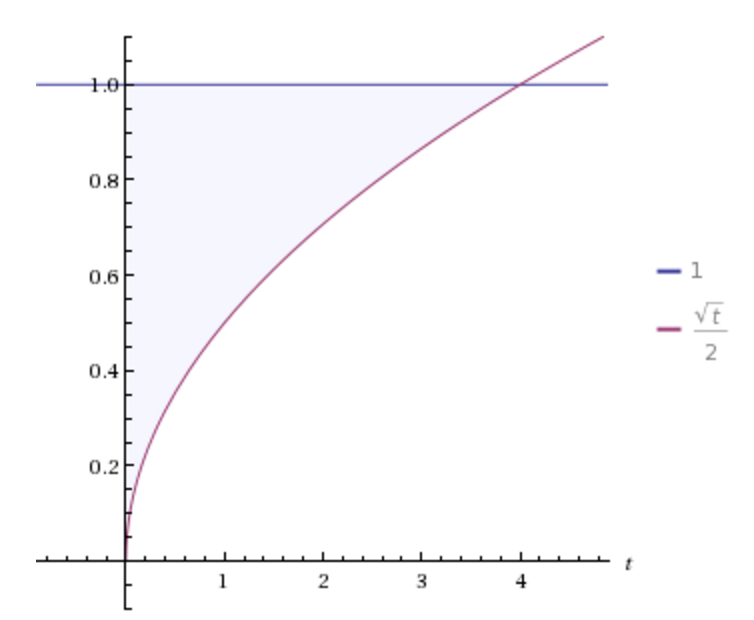
\includegraphics[width=0.5\textwidth]{graphic1.png}
        \end{center}
      }
    }

    \subproblem{}{
      Calculate the Speed Index of our webapp.

      \solution{
        \begin{align*}
          \text{SpeedIndex}
          &= \int_0^4 1 - L(t) \, dt \\
          &= \int_0^4 1 - \frac{1}{2}t^{1/2} \, dt \\
          &= \left[ t - \frac{1}{3}t^{3/2} \right]_0^4 \\
          &= 1.\bar{3}
        \end{align*}
      }
    }
  \end{problem}

  \begin{problem}{}
    Our engineers must design a loading function $L(t)$, and they must
    optimally decide between two trade-offs as follows. Our loading
    function $L(t)$ is piecewise linear with one segment connecting
    $(0,0)$ and $\left( \frac{1}{3x}, \frac{1}{2} \right)$ and with the
    other segment connecting $\left( \frac{1}{3x}, \frac{1}{2} \right)$
    and $(x,1)$ (illustrated below).

    \begin{center}
      % DESCRIPTION:
% KEYWORDS:
\documentclass[border=0.5in]{standalone}

\usepackage{fbpicture}

\begin{document}
  \begin{fbpic}{-1}{5}{-1}{3}
    % \putframe\relax
    % \putgridlines\relax
    \linethickness{1pt}
    % axes
    \putaxes\relax
    % \put(5.2,-0.1){$x$}
    % \put(-0.1,5.2){$y$}
    % \put(0.7,0.1){$1$}
    % \put(0.1,0.7){$1$}
    % functions
    \put(0,0){\circle*{0.1}}
    \put(0.1,-0.4){$(0,0)$}
    \put(0.5,1){\circle*{0.1}}
    \put(0.6,0.6){$\left( \frac{1}{3x}, \frac{1}{2} \right)$}
    \put(4,2){\circle*{0.1}}
    \put(4.1,1.9){$(x, 1)$}
    \put(0,0){\line(0.5,1){0.5}}
    \put(0.5,1){\line(3.5,1){3.5}}
    \put(-0.5,2){$1$}
    \put(-0.5,1){$\frac{1}{2}$}
  \end{fbpic}
\end{document}

    \end{center}

    Notice that choosing a large value for $x$ will speed up the loading
    of the first half of our webapp, but at the cost of increasing
    the overall loading time of our webapp. It is not clear whether we
    should choose a small number for $x$ or a large number for $x$.

    Our engineers must optimally pick the value of $x$ so that the
    Google Speed Index of our webapp is minimized (Twitter recently
    made a similar analysis to optimize the loading time of their
    main page).

    \subproblem{}{
      Find the Speed Index of $L(t)$ in terms of $x$.

      \hint{Use Geometry}

      \solution{
        \begin{align*}
          \text{SpeedIndex}
          &= \int_0^x 1 - L(t) \, dt \\
          &= \int_0^{\frac{1}{3x}} 1 - L(t) \, dt
            + \int_{\frac{1}{3x}}^x 1 - L(t) \, dt \\
          &= \left(\frac{1}{2}\right)\left(\frac{1}{3x}\right)
            + \left(\frac{1}{2}\right)
              \left(\frac{1}{2}\right)
              \left(\frac{1}{3x}\right)
            + \left(\frac{1}{2}\right)
              \left(\frac{1}{2}\right)
              \left(x - \frac{1}{3x}\right) \\
          &= \frac{1}{6}x^{-1} + \frac{1}{4}x
        \end{align*}
      }
    }

    \subproblem{}{
      Pick $x$ so that the Speed Index of $L(t)$ is minimized.

      \solution{
        \begin{align*}
          \text{SpeedIndex}(x) &= \frac{1}{6}x^{-1} + \frac{1}{4}x \\
          \text{SpeedIndex}'(x) &= - \frac{1}{6}x^{-2} + \frac{1}{4} \\
          \text{SpeedIndex}''(x) &= \frac{1}{3}x^{-3}
        \end{align*}

        Find any stationary points.

        \begin{gather*}
          0 = \text{SpeedIndex}'(x) \\
          0 = - \frac{1}{6}x^{-2} + \frac{1}{4} \\
          \pm \sqrt{\frac{2}{3}} = x \\
        \end{gather*}

        We reject $-\sqrt{\frac{2}{3}}$, since a negative value for $x$
        does not make sense for our purpose.

        To see that $\sqrt{\frac{2}{3}}$ is a local minimum, we check
        the concavity of $\text{SpeedIndex}(x)$ at $\sqrt{\frac{2}{3}}$.

        \[
          \text{SpeedIndex}''\left(\sqrt{\frac{2}{3}}\right)
          = \frac{1}{3}\left(\sqrt{\frac{2}{3}}\right)^{-3}
          > 0
        \]

        The concavity is positive, so $\sqrt{\frac{2}{3}}$ produces
        a local minimum.
      }
    }
  \end{problem}

\end{document}
